\chapter{Organisation générale de l'application}

\section{Importation des modules}

	Notre programme consistant principalement en des instances de classes qui interragissent entre elles, nous avons décidé de séparer notre code avec un fichier par classe.

	\begin{figure}[H]
		\centering
		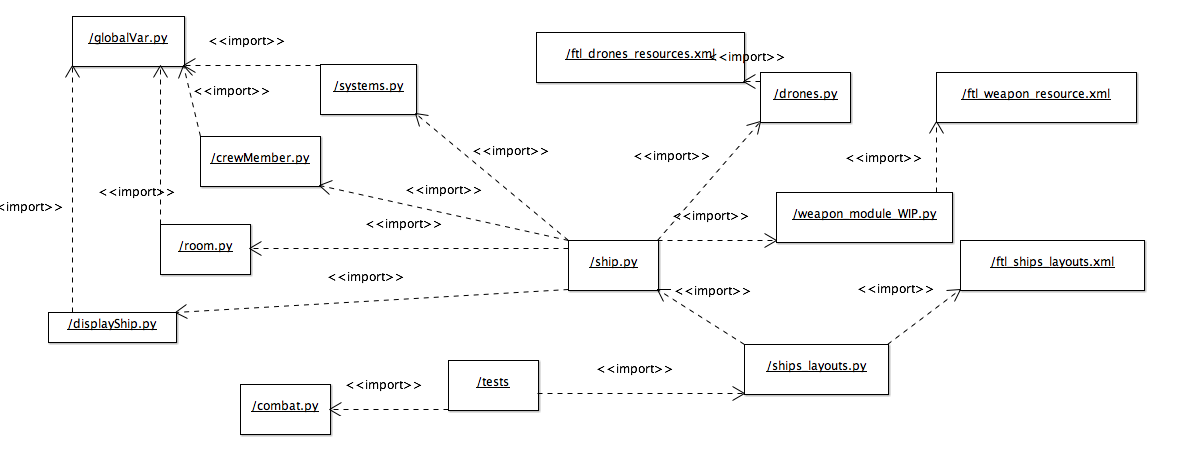
\includegraphics[width=1\linewidth]{smoothPackageDiagram}
	\end{figure}
	
	Comme nous pouvons le voir sur le graphique, le programme est lancé par les modules de tests (test-combats et tournament-test) qui importent combat qui est simplement la fonction qui lance un combat. De plus les tests ont besoin de générer un vaisseau, et c'est là que l'arboresence se complique car le vaisseau est contitué de nombreuses classes (une classe est représenté par un module), et a besoin de plusieurs fichiers xml.


\section{Diagramme des classes et représentation des vaisseaux}

	\begin{figure}[H]
		\centering
		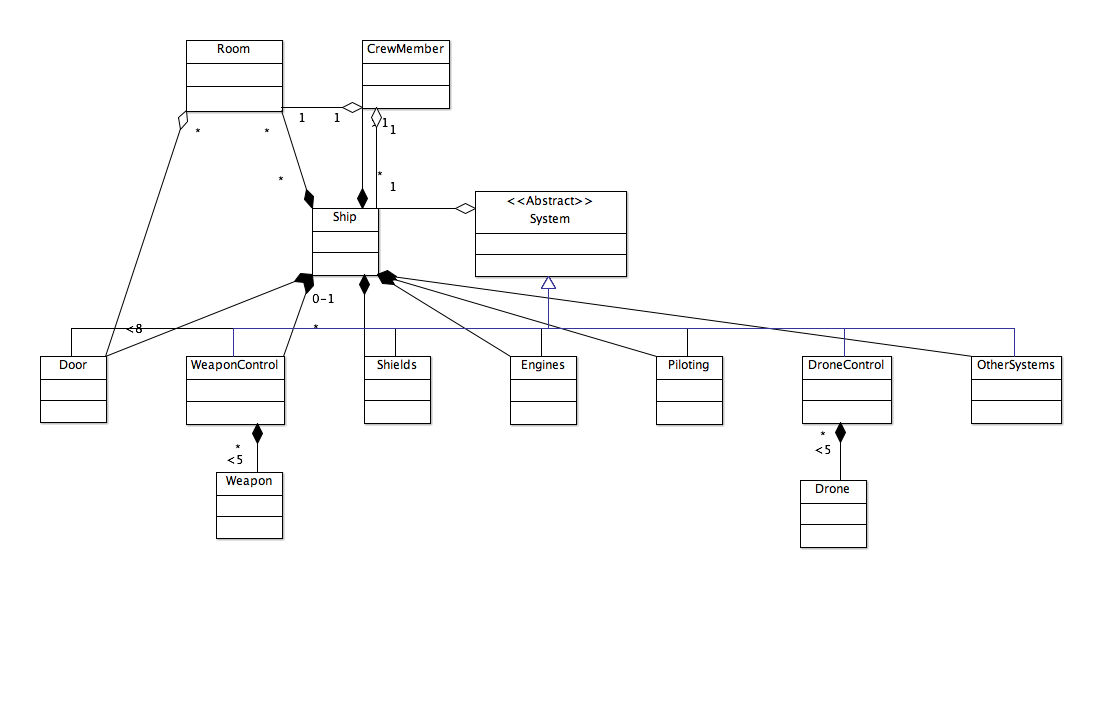
\includegraphics[width=1\linewidth]{smoothUmlDiagram}
	\end{figure}

	Toutes les classes ont un rapport direct avec la représentation d'un vaisseau. Le diagramme montre donc la représentation d'un vaisseau qui se décompose ainsi :\\
	\begin{itemize}
	\item Un vaisseau contient des systèmes, des salles et des membres d'équipage. 
	\item Les drones et armes appartiennent à leurs systèmes respectifs.
	\item Les systèmes et membres d'équipage ont aussi le vaisseau en attribut car ils agissent souvent sur le vaisseau.
	\item Les membres d'équipage possèdent la salle dans laquelle ils sont.
	\item Les salles possèdent des portes.
	\end{itemize}


\section{Stockage des données}

	Comme dit précédement, les données issues du jeu original sont mises dans des fichiers xml.	Ces données concernent les vaisseaux de base, les armes et drones.\\
	
	L'importation des données inscrites dans les fichiers xml sont extraites grâce au module python xml.etree.ElementTree
	
	Pour les vaisseaux, nous avons stocké les données suivantes :
	\begin{itemize}
		\item Les systèmes présents et leurs énergies de base.
		\item Les armes et les drones.
		\item Les salles avec : leurs coordonnées, le système qui est dedans ou celui qui peut être dedans, les portes, les membres d'équipage.
	\end{itemize}
	Pour les armes et drones, nous avons stocké les temps de rechargement et d'autres informations qui dépendent de chaque objet.
	

\section{Le déroulement d'un combat}

Nous avons décidé de gérer un combat avec un fonctionnement au tour-par-tour tout en gardant un faible temps entre chaque tour. 
Cela nous permet de gérer les phases d'attaques et de cooldowns indépendamment, tout en restant proche du jeu original qui est en temps réel.	

	
	\subsection{Le déroulement d'une attaque}

		L'utilisation d'une arme :\\
		Pour chaque arme, la même procédure va être appliquée. Celle-ci est gérée par le système des armes.
		\begin{figure}[H]
			\centering
			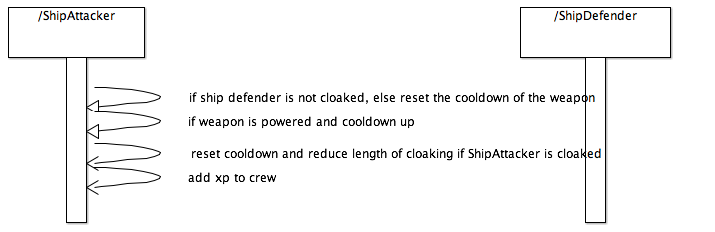
\includegraphics[width=1\linewidth]{smoothUseWeaponToAttackSequenceDiagramStart}
		\end{figure}
		Le système fait d'abord tous les préparatifs avant d'être sûr qu'il a le droit d'utiliser l'arme. Ensuite si toutes les conditions sont remplies, il l'utilise. Les différents types d'armes ont des fonctionnements différents.
		\begin{figure}[H]
			\centering
			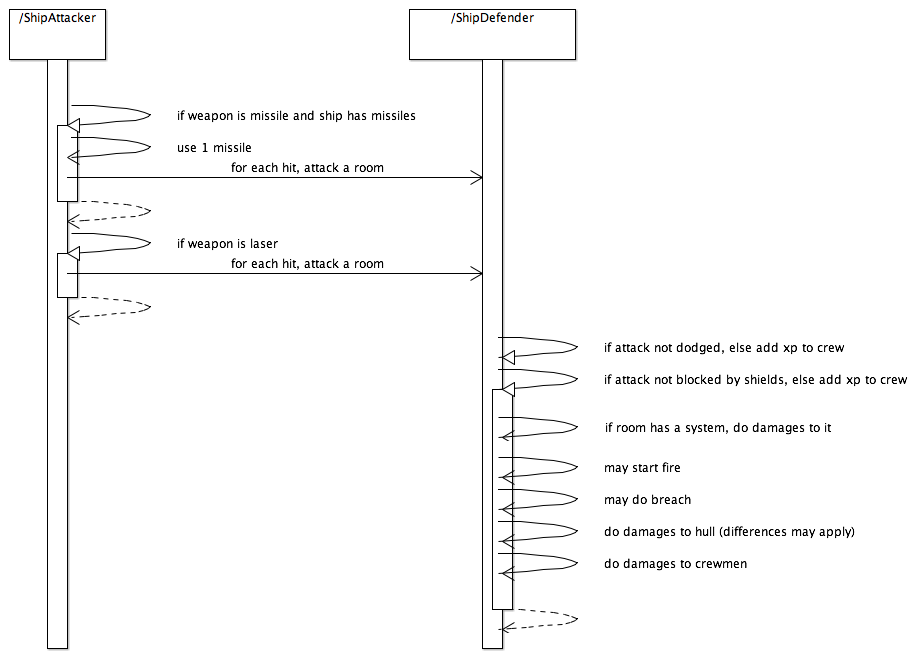
\includegraphics[width=1\linewidth]{smoothUseWeaponToAttackSequenceDiagramMissileLaser}
		\end{figure}
		Les armes lasers et missiles ont des fonctionnements similaire, il faut seulement s'assurer de la bonne gestion des missiles. Ensuite la même méthode du vaisseau adverse est appelée. \\
		Celle-ci manipule d'abord l'esquive et les boucliers. Ensuite, si l'attaque est passée, des dégats sont appliqués aux systèmes, aux membres d'équipage présents dans la salle, à la coque (hull) et des départs de feu ou des brèches peuvent être générés. 
		\begin{figure}[H]
			\centering
			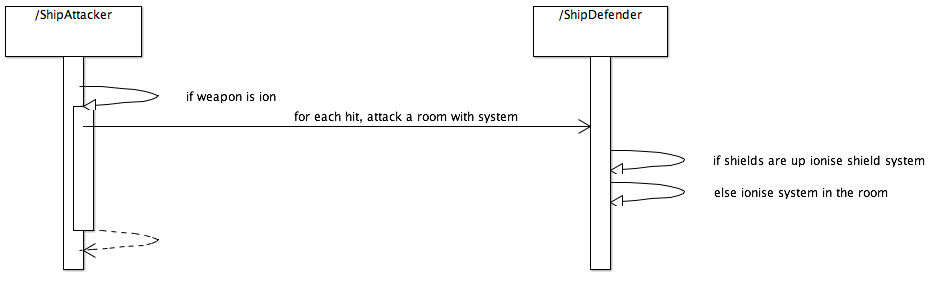
\includegraphics[width=1\linewidth]{smoothUseWeaponToAttackSequenceDiagramIon}
		\end{figure}
		Les armes ions font des dégats temporaires aux systèmes et seulement à eux.\\
		Pour utiliser ces armes, il suffit donc d'appeler la méthode du vaisseau adverse. Celle-ci va juste se contenter de d'ioniser les boucliers s'il y a une couche de bouclier opérationnelle, sinon ioniser le système visé originellement.
		\begin{figure}[H]
			\centering
			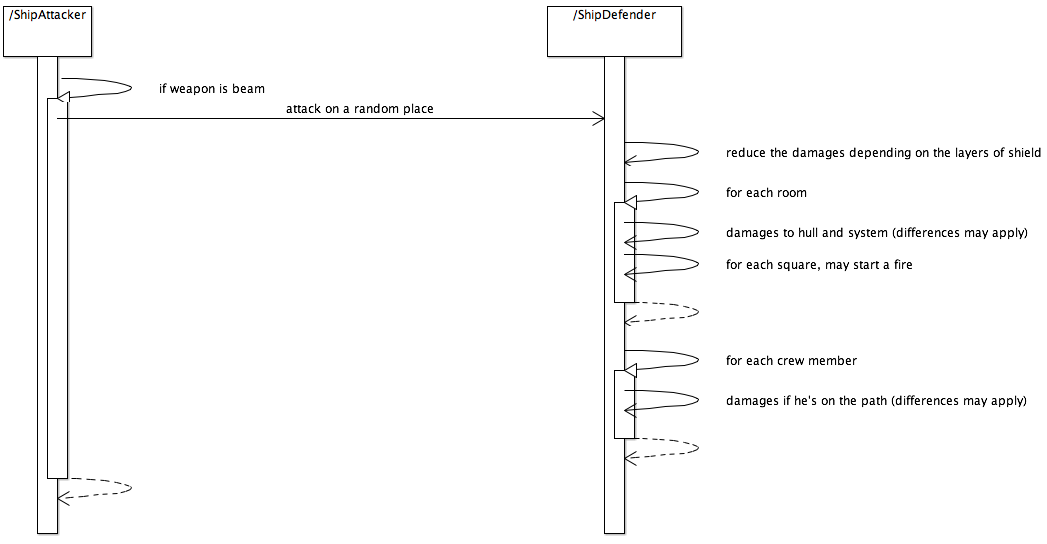
\includegraphics[width=1\linewidth]{smoothUseWeaponToAttackSequenceDiagramBeam}
		\end{figure}
		Les rayons font des dégats sur une ligne dans le vaisseau grâce à des coordonnées aléatoires.\\
		La méthode du vaisseau adverse devra donc faire des dégats à tout ce qui se trouve sur le chemin du rayon.

	\subsection{La gestion des cooldowns}

		Le vaisseau :
  		L'ordre des différentes instruction n'a pas vraiment d'importance. Nous allons donc lister ces instructions : \\
		\begin{enumerate}
			\item Demander aux systèmes de gérer leurs cooldowns.
    	\item Essayer d'alimenter les differents systèmes, armes et drones.
			\item Annuler les réparations efféctuées d'un système s'il n'y a plus personne dans la salle.
			\item Demander aux salles de gérer leurs cooldowns.
     	\item Demander aux membres d'équipage de gérer leurs déplacements (Cette partie ne fonctionnant pas très bien, et n'étant pas la priorité du programme, nous avons décidé de mettre cet élément du jeu en pause).
			\item Ajouter de l'oxygène aux salles grâce au système.
			\item Essayer d'utiliser l'invisibilité.
		\end{enumerate}

		\medskip

		Les systèmes :
		Tous les systèmes doivent gérer le cooldown de leur ionisation.\\
		Le système des boucliers doit gérer le cooldown de ses couches de bouclier.\\
		Les systèmes des armes et des drones doivent recharger respectivement les armes et les drones.
		\medskip

		Les salles :
		\begin{enumerate}
			\item Gérer les différentes tâches des membres d'équipage présents (réparation, extinction...).
			\item Gérer les dégâts faits aux membres d'équipage.
			\item Gérer le reste de l'oxygène.
			\item Gérer les feux et les brèches.
		\end{enumerate} 
